\documentclass[serif,mathserif,final]{beamer}
\mode<presentation>{\usetheme{Lankton}}
\usepackage{amsmath,amsfonts,amssymb,pxfonts,eulervm,xspace}
\usepackage{framed,graphicx}
\usepackage{kky}
\graphicspath{{./figures/}}
\usepackage[orientation=landscape,size=custom,width=78,height=95,scale=.6,debug]{beamerposter}

%-- Header and footer information ----------------------------------
\newcommand{\footleft}{keywords: Gibbs Sampling, Markov Networks, Mixing Times}
\newcommand{\footright}{ \{wenluh, kkandasa, jtassro\} @ cs.cmu.edu }
\title{Improving Mixing times in Gibbs Sampling}
\author{Wenlu Hu \quad Kirthevasan Kandasamy \quad Joseph Tassarotti}
\institute{10-701 Introduction to Machine Learning, Course Project}
%-------------------------------------------------------------------


%-- Main Document --------------------------------------------------
\begin{document}
\begin{frame}{}
  \begin{columns}[t]

    %-- Column 1 ---------------------------------------------------
    \begin{column}{0.49\linewidth}

      %-- Block 1-1
      \begin{block}{Summary}
        This is a poster containing text and other things
        This part is the summary.  People might read this
      \end{block}

      %-- Block 1-2
      \begin{block}{Motivation}
        You can make a poster very quickly and easily by cutting and pasting
        the \LaTeX~codes from the paper!
      \end{block}

      %-- Block 1-3
      \begin{block}{Columns}
        The columns will automatically align with each other and try to look
        as nice as possible.  You may have to add {\tt$\backslash$vspace\{1pt\}}
        commands to adjust the spacing here and there.  Remember that you can
        use positive or negative numbers.
      \end{block}

      %-- Block 2-?
      \begin{block}{Algorithms}
		For tree splitting, we consider algorithm from \cite{}. They
		greedily grows trees favoring vertices of low degree. We use
		its slightly simplified version as our baseline. We compared
		our algorithm, Greedy Edge Selection Algorithm, with the
		baseline under two different conditions.
		%\hsize .5\columnwidth
		\begin{columns}[t]
			%-- Column for algo
			\begin{column}{0.49\linewidth}

\begin{framed}
\noindent\textbf{Greedy Edge Selection Algorithm}
\begin{enumerate}
\item Construct an ordered list of edges, $E$, with $E[0]$ being the highest weight edge. Edges are vertex pairs $(i,j)$.
\item Initialize an all-zero $n$-dimensional integer list $V$ of vertex colors. \\
($V[i]$ is the color of vertex $i$, and $V[i]=0$ means that vertex $i$ has not yet been colored.)
\item Initialize $n$ empty vertex sets: $T_1,...,T_n$\\
(Logically, $T_i$ is the set of vertices labeled with color $i$.)
\item Initialize $unusedColor=1$.
\item For each edge $e=(i,j)$ in $E$,
\begin{itemize}
\item If $V[i]=V[j]=0$,
\begin{itemize}
\item Set $V[i]=V[j]=unusedColor$
\item Add $i,j$ to $T_{unusedColor}$
\item Increment $unusedColor$ by $1$
\end{itemize}
\item Else if $V[i]=0$ and $V[j]\notin getOtherNeighborColors(\{i\}, e)$,
\begin{itemize}
\item Set $V[i]=V[j]$
\item Add $i$ to $T_{V[j]}$
\end{itemize}
\item Else if $V[j]=0$ and $V[i]\notin getOtherNeighborColors(\{j\}, e)$,
\begin{itemize}
\item Set $V[j]=V[i]$
\item Add $j$ to $T_{V[i]}$
\end{itemize}
\item Else if  $V[i]\neq 0$ and $V[j]\neq 0$ and $V[i]\notin getOtherNeighborColors(T_j, e)$,
\begin{itemize}
\item For each $k\in T_j$, set $V[k]=V[i]$
\item Set $T_i=T_i\cup T_j$
\item Set $T_j=\emptyset$
\end{itemize}
\item Otherwise do nothing
\end{itemize}
\item For each vertex $i$, if $V[i]=0$, set $V[i]=unusedColor$, $unusedColor++$
\item Output $\{T_j:T_j\neq\emptyset\}$
\end{enumerate}
\end{framed}

\begin{framed}
\noindent\textbf{Greedy Tree Growing Algorithm} % \cite{rivasseau2005jungle}}
\begin{enumerate}
\item Initialize $i=0$ and $V$ to the vertex set.
\item While $V\neq\emptyset$
\begin{itemize}
\item Select $v\in V$
\item Start a new tree $T_i$ and a priority queue $Q_i$. Add $v$ to $Q_i$
\item While $Q_i\neq\emptyset$
\begin{itemize}
\item Pop $u$ from $Q_i$.
\item Initialize $neighborsInT=0$.
\item For all $v\in T_i$, if $u\in N(v)$, increment $neighborsInT$
\item If $neighborsInT\le1$,
\begin{itemize}
\item Add $u$ to $T_i$ and remove $v$ from $V$
\item Add $N(u)$ to $Q_i$.
\end{itemize}
\end{itemize}
\end{itemize}
\item Return $\{T_i\}$
\end{enumerate}
\end{framed}

			\end{column}
			%-- Column for algo
			\begin{column}{0.49\linewidth}

\begin{figure}
	\centering
	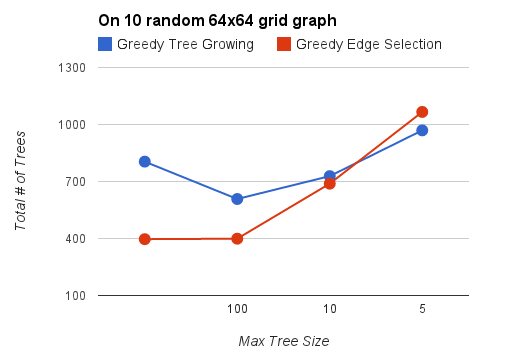
\includegraphics[width=\columnwidth]{TotalTrees-Vs-MaxTreeSize.png}
\end{figure}
\vspace{-0.4in}
\begin{figure}
	\centering
	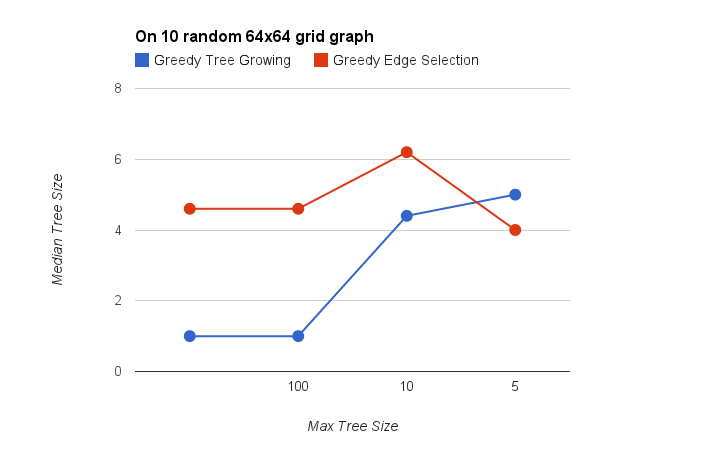
\includegraphics[width=\columnwidth]{MedianTreeSize-Vs-MaxTreeSize.png}
\end{figure}
\vspace{-0.4in}

%			We consider a tree-splitting algorithm to be good if it
%			can give us a small number of total trees and if the
%			median size of the trees are relatively small. 
			
			With no limit on the max tree size (the leftmost dots),
			Greedy Edge Selection Algorithm performs much better than
			Greedy Tree Growing Algorithm. 

			But when as the limit of max tree size goes down, Greedy
			Tree Growing Algorithm caught up with Greedy Edge
			Selection Algorithm.
			\end{column}
		\end{columns}

      \end{block}

    \end{column}%1

    %-- Column 2 ---------------------------------------------------
    \begin{column}{0.49\linewidth}

      %-- Block 2-1
      \begin{block}{Lists}
        \begin{itemize}
          \item You can make
          \item lists, that
          \item allow people to see quickly
        \end{itemize}
      \end{block}

      %-- Block 2-2
      \begin{block}{Math}
        Include math within the text is as simple as $1+1=2$.  You can also
        highlight more important equations like this:
        \begin{equation*}
          \int_0^1\sin(x)+\cos^2(x)+\alpha x~d\!x
        \end{equation*}
      \end{block}


      %-- Block 2-3
      \begin{block}{Pictures}
        \begin{figure}[htb]
          \centering
%           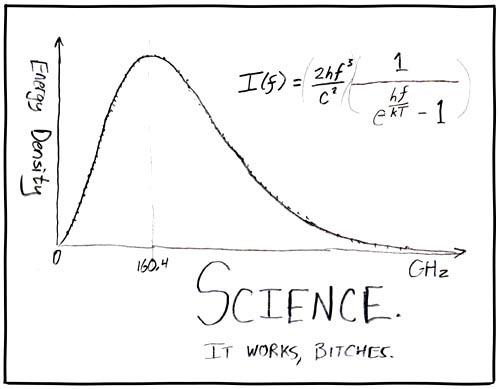
\includegraphics[width=.6\columnwidth]{science}
        \end{figure}
      \end{block}

      %-- Block 3-1
      \begin{block}{Experiments}
        Remember to put lots of figures on your poster... Nobody reads anymore!
      \end{block}

      %-- Block 3-2
      \begin{block}{Conclusion}
        Much less annoying than PowerPoint.  Copy and Paste from your
        document. Overall, a great idea!
      \end{block}

    \end{column}%2

% I think we should do just 2 columns
%     %-- Column 3 ---------------------------------------------------
%     \begin{column}{0.32\linewidth}
% 
%     \end{column}%3

  \end{columns}
\end{frame}
\end{document}
